\section{定积分的应用 II}

\subsection{求平面图形面积 continue}

\subsubsection{参数方程情形}

若曲边梯形的曲边由参数方程
$$
\begin{cases}
	x = \varphi(t)\\
	y = \psi(t)
\end{cases}, (t \in [t_1, t_2])
$$
决定,且在 $[t_1, t_2]$ 上,$\varphi(t)$ 有连续导数,$\varphi(t_1) \neq 0$,$\psi(t)$ 连续,那么曲边梯形的面积为:
$$
A = \int_{t_1}^{t_2} |\psi(t) \,\dd \varphi(t)| = \int_{t_1}^{t_2} |\psi(t) \varphi'(t)| \dd{t}
$$

\subsubsection{极坐标情形}

要求极坐标下的曲线 $r = \varphi(\theta)\ (\theta \in [\alpha, \beta], [\alpha, \beta] \subseteq [0, 2 \pi])$ 与直线 $y = x \tan \alpha,\ y = x \tan \beta$ 围成的图形的面积,可以取小扇形作为微元:

\begin{figure}[H]
	\centering
	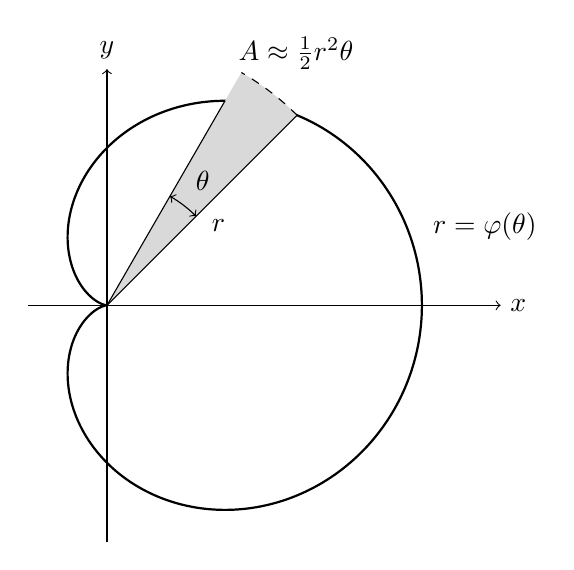
\begin{tikzpicture}[scale=2]
		% Draw axes
		\draw[->] (-0.5,0) -- (2.5,0) node[right] {$x$};
		\draw[->] (0,-1.5) -- (0,1.5) node[above] {$y$};
		
		% Define the cardioid function r = a(1 + cos(theta)), let a=1
		\draw[thick, domain=0:360, samples=200, smooth] plot ({ (1 + cos(\x)) * cos(\x) }, { (1 + cos(\x)) * sin(\x) });
		
		% Draw the sector (differential element)
		\def\angleA{45}
		\def\angleB{60}
		\pgfmathsetmacro{\radiusA}{1 + cos(\angleA)}
		\pgfmathsetmacro{\radiusB}{1 + cos(\angleB)}
		
		% Fill the sector
		\fill[gray!30] (0,0) -- (\angleA:\radiusA) arc (\angleA:\angleB:\radiusA) -- cycle;
		
		% Draw the rays for the sector
		\draw (0,0) -- (\angleA:\radiusA) node[midway, below right] {$r$};
		\draw (0,0) -- (\angleB:\radiusB);
		
		% Draw the arc approximation
		\draw[dashed] (\angleA:\radiusA) arc (\angleA:\angleB:\radiusA);
		
		% Label the differential angle
		\draw[<->] (\angleA:0.8) arc (\angleA:\angleB:0.8);
		\node at (52.5:1.0) {$\dd \theta$};

		% Label the curve
		\node at (2.4, 0.5) {$r = \varphi(\theta)$};
		
		% Label the area element
		\node at (1.2, 1.6) {$\dd A \approx \frac{1}{2} r^2 \dd \theta$};
	\end{tikzpicture}
	\caption{极坐标系下曲边扇形的面积微元}
\end{figure}

得到图形面积为:
$$
A = \int_\alpha^\beta \frac{1}{2} \varphi(\theta)^2 \,\dd \theta
$$

\subsection{立体图形的体积}

\subsubsection{$y = f(x)$ 绕 $x$ 轴旋转}

要求连续曲线 $y = f(x)$、直线 $x = a$、直线 $x = b$、$x$ 轴围成的图形,绕 $x$ 轴旋转一周得到的旋转体,我们可以使用圆盘作为微元:

\begin{figure}[H]
	\centering
	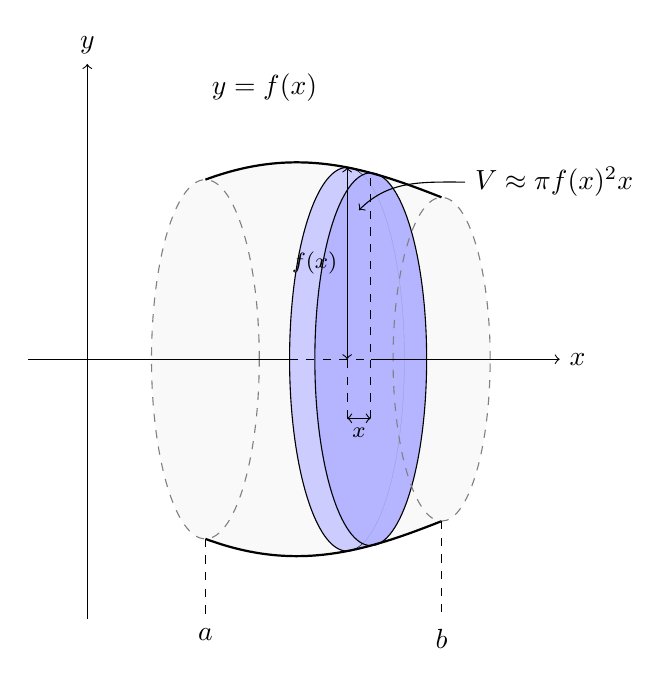
\begin{tikzpicture}[scale=1.5]
		% Definitions
		\def\f#1{(1 + 0.5*sin((#1) r) + 0.1*(#1))}
		\def\xa{1}
		\def\xb{3}
		\def\xscale{0.3}
		\def\xslice{2.2}
		\def\dx{0.2}
		
		% Calculate key points
		\pgfmathsetmacro{\ra}{\f{\xa}}
		\pgfmathsetmacro{\rb}{\f{\xb}}
		\pgfmathsetmacro{\rslice}{\f{\xslice}}
		\pgfmathsetmacro{\rnext}{\f{\xslice+\dx}}
		\pgfmathsetmacro{\xr}{\xscale*\rslice}
		\pgfmathsetmacro{\xrr}{\xscale*\rnext}

		% 2. Main Body Fill (Background)
		\fill[gray!5] plot[domain=\xa:\xb, samples=100] (\x, {\f{\x}})
					  arc (90:-90:{\xscale*\rb} and {\rb})
					  plot[domain=\xb:\xa, samples=100] (\x, {-\f{\x}})
					  arc (-90:-270:{\xscale*\ra} and {\ra}) -- cycle;

		% 3. Back Face
		\draw[dashed, gray] (\xa,0) ellipse ({\xscale*\ra} and {\ra});

		% 4. Disk (Volume Element)
		% Back Ellipse of Disk
		\draw[fill=blue!20] (\xslice,0) ellipse ({\xr} and {\rslice});
		% \fill[blue!20] (\xslice,-\rslice) -- (\xslice,\rslice) -- (\xslice+\dx,\rnext) -- (\xslice+\dx,-\rnext) -- cycle;
		
		% Disk Side (using exact curves)
		\fill[blue!20] plot[domain=\xslice:\xslice+\dx, samples=100] (\x, {\f{\x}})
					   arc (90:-90:{\xrr} and {\rnext})
					   plot[domain=\xslice+\dx:\xslice, samples=100] (\x, {-\f{\x}})
					   arc (-90:90:{\xr} and {\rslice}) -- cycle;
					   
		% % Side lines (Top and Bottom only)
		\draw[blue!60!black] plot[domain=\xslice:\xslice+\dx, samples=10] (\x, {\f{\x}});
		\draw[blue!60!black] plot[domain=\xslice:\xslice+\dx, samples=10] (\x, {-\f{\x}});

		% Front Ellipse of Disk
		\draw[fill=blue!30, fill opacity=0.9] (\xslice+\dx,0) ellipse ({\xrr} and {\rnext});

		% 5. Main Body Outline (Foreground)
		\draw[thick] plot[domain=\xa:\xb, samples=100] (\x, {\f{\x}});
		\draw[thick] plot[domain=\xa:\xb, samples=100] (\x, {-\f{\x}});
		
		% Front Face of Solid
		\draw[dashed, gray] (\xb,0) ellipse ({\xscale*\rb} and {\rb});
		
		% 6. Annotations
		\node at (1.5, 2.3) {$y=f(x)$};
		
		% x-limits labels
		\draw[dashed] (\xa, -\ra) -- (\xa, -2.2) node[below] {$a$};
		\draw[dashed] (\xb, -\rb) -- (\xb, -2.2) node[below] {$b$};
		
		% Element labels
		% f(x) radius - move to the right side of the disk to avoid overlap with back lines
		\draw[<->] (\xslice, 0) -- (\xslice, \rslice) node[midway, left, font=\footnotesize] {$f(x)$};
		
		% dx label
		\draw[<->] (\xslice, -0.5) -- (\xslice+\dx, -0.5); 
		\node[below, font=\footnotesize] at (\xslice+0.5*\dx, -0.5) {$\dd x$};
		\draw[dashed, thin] (\xslice, -0.5) -- (\xslice, 0);
		\draw[dashed, thin] (\xslice+\dx, -0.5) -- (\xslice+\dx, \rnext);
		
		% dV label - move higher and use a cleaner arrow
		\draw[->] (3.2, 1.5) node[right, align=left] {$\dd V \approx \pi f(x)^2 \dd x$} to[out=180, in=45] (\xslice+0.5*\dx, 0.8*\rnext);

		% 1. Draw Axis (Background parts)
		\draw (-0.5,0) -- (\xslice-\xr,0); % Solid before disk
		\draw[dashed] (\xslice-\xr,0) -- (\xslice+\dx,0); % Dashed behind disk
		\draw[->] (\xslice+\dx,0) -- (4,0) node[right] {$x$}; % Solid after disk with Arrow
		\draw[->] (0,-2.2) -- (0,2.5) node[above] {$y$};
	\end{tikzpicture}
	\caption{旋转体体积微元(圆盘法)}
\end{figure}

得到体积为:
$$
V = \pi \int_a^b f(x)^2 \dd{x}
$$

\subsubsection{$x = f(y)$ 绕 $y$ 轴旋转}

与上面同理,面积为:
$$
V = \pi \int_a^b f(y)^2 \dd{y}
$$

\subsubsection{$y = f(x)$ 绕 $y$ 轴旋转}

要求连续曲线 $y = f(x)$、直线 $x = a$、直线 $x = b$、$x$ 轴围成的图形,\textbf{绕 $y$ 轴}旋转一周得到的旋转体,体积为:
$$
V = 2\pi \int_a^b x |f(x)| \dd{x}
$$

\subsubsection{截面面积已知的立体图形体积}

若在平面 $x = a, x = b$ 之间的立体图形,由平面 $x = t$ 截出的面积为 $f(t)$,那么图形的体积为:
$$
V = \int_a^b f(t) \dd{t}
$$

\subsubsection{极坐标下旋转体的体积}

要求一个极坐标曲线 $\rho = f(\theta)$ 绕极轴旋转得到的旋转体,可以使用微元法加上重心的方法。对于一个半径为 $r$ 的微小扇形,其重心离圆心的距离为 $\frac{2}{3} r$,重心移动的距离为 $\frac{2\pi}{3} r \sin \theta$,那么得到整个图形的体积:
$$
V = \frac{2\pi}{3}\int_\alpha^\beta f(\theta)^3 \sin \theta \,\dd \theta
$$

\subsection{求曲线的弧长}

\subsubsection{$y = f(x)$ 的弧长}

对于曲线 $y = f(x),\ (x \in [a, b])$,使用微元法:

\begin{figure}[H]
	\centering
\begin{tikzpicture}[scale=1.5, >=stealth]
		% Axes
		\draw[->] (-0.5,0) -- (3.5,0) node[right] {$x$};
		\draw[->] (0,-0.5) -- (0,3.5) node[above] {$y$};
		
		% 1. Function Definition and Variables
		\def\f#1{-0.2*(#1)^3 + 0.5*(#1)^2 + 0.8*#1 + 0.5} % A cubic function example
		\def\xa{1.5}    % Start x of the element
		\def\dx{0.8}    % Width of element dx
		\def\xmin{0.2}  % Plot domain start
		\def\xmax{3.0}  % Plot domain end
		
		% 2. Calculate coordinates
		\pgfmathsetmacro{\ya}{\f{\xa}}          % y at x
		\pgfmathsetmacro{\xb}{\xa + \dx}        % x + dx
		\pgfmathsetmacro{\yb}{\f{\xb}}          % y at x + dx
		
		% 3. Draw Main Curve
		\draw[thick, name path=curve] plot[domain=\xmin:\xmax, samples=100, smooth] (\x, {\f{\x}}) node[right] {$y=f(x)$};
		
		% 4. Draw Differential Triangle
		\coordinate (A) at (\xa, \ya);
		\coordinate (B) at (\xb, \yb);
		\coordinate (C) at (\xb, \ya); % Right angle vertex
		
		% dx and dy sides
		\draw[dashed] (A) -- (C) node[midway, below] {$\dd x$};
		\draw[dashed] (C) -- (B) node[midway, right] {$\dd y$};
		
		% Hypothenuse (Chord approximations ds)
		\draw[red] (A) -- (B);
		
		% 5. Highlight the Arc Element
		\draw[blue, very thick] plot[domain=\xa:\xb, samples=50] (\x, {\f{\x}});
		\node[blue, above right] at (\xa + 0.3*\dx, \ya + 0.4) {$\dd s$};
		
		% 6. Points
		\fill (A) circle (1.5pt);
		\fill (B) circle (1.5pt);
		
		% 8. Axis projections (Optional, but good for clarity)
		\draw[dashed, thin, gray] (A) -- (\xa, 0) node[below, black] {$x$};
		\draw[dashed, thin, gray] (C) -- (\xb, 0) node[below, black] {$x+\dd x$};
		
	\end{tikzpicture}
	\caption{弧长微元示意图}
\end{figure}

得到弧长为:
$$
s = \int_a^b \dd s = \int_a^b \sqrt{\dd y^2 + \dd x^2} = \int_a^b \sqrt{1 + f'(x)^2} \dd x
$$

\subsubsection{参数方程情形}

对于参数曲线:
$$
\begin{cases}
	x = \varphi(t)\\
	y = \psi(t)
\end{cases}, \quad t \in [a, b]
$$
使用类似的微元分析,可以得到:
$$
s = \int_a^b \sqrt{\dd \varphi(t)^2 + \dd \psi(t)^2} = \int_a^b \sqrt{\varphi'(t)^2 + \psi'(t)^2} \dd{t}
$$

\subsubsection{极坐标情形}

对于极坐标下的曲线 $r = f(\theta),\ \theta \in [\alpha, \beta]$,我们可以将其视作参数方程:
$$
\begin{cases}
	x = f(\theta) \cos \theta\\
	y = f(\theta) \sin \theta
\end{cases}, \quad \theta \in [\alpha, \beta]
$$
于是得到弧长为:
$$
s = \int_\alpha^\beta \sqrt{f(\theta)^2 + f'(\theta)^2} \, \dd \theta
$$

\subsection{作业}

\begin{problem}
	课后习题 7.3.1

	\begin{solution}
		\begin{enumerate}
			\item[\textbf{2)}] 
			$$
			\begin{aligned}
				\text{原式} & = \lim_{n \to \infty} \sum_{k=1}^n \frac{n^2}{(n + k)^2} \cdot \frac{1}{n} \\
				& = \lim_{n \to \infty} \frac{1}{\ab(1 + \frac{k}{n})^2} \cdot \frac{1}{n} \\
				& = \int_0^1 \frac{1}{(1 + x)^2} \dd x \\
				& = \ab[-\frac{1}{1 + x}]_0^1 = \frac{1}{2}
			\end{aligned}
			$$

			\item[\textbf{4)}]
			$$
			\begin{aligned}
				\text{原式} & = \lim_{n \to \infty} \sum_{k=1}^n \ab(1 + \frac{k}{n}) \ab(\frac{k \pi}{n^2} + O\ab(\frac{k^3 \pi^3}{n^6})) \\
				& = \lim_{n \to \infty} \sum_{k=1}^n \ab(1 + \frac{k}{n}) \frac{k \pi}{n^2} \\
				& = \lim_{n \to \infty} \ab(1 + \frac{k}{n}) \frac{k}{n} \cdot \frac{1}{n} \\
				& = \int_0^1 (1 + x) x \dd{x} \\
				& = \ab[\frac{1}{2} x^2 + \frac{1}{3} x^3]_0^1 = \frac{5}{6}
			\end{aligned}
			$$
		\end{enumerate}
	\end{solution}    
\end{problem}

\begin{problem}
	课后习题 7.3.2

	\begin{solution}
		\begin{enumerate}
			\item[\textbf{2)}] 由题可知:
			$$
			\int_0^x \E^{t^2} \dd{t} > x \cdot \E^0 = x \\
			\int_0^x \E^{2 t^2} \dd{t} > x \cdot \E^0 = x
			$$
			因此 $x \to \infty$ 时,$\int_0^x \E^{t^2} \dd{t} \to \infty,\ \int_0^x \E^{2 t^2} \dd{t} \to \infty$。

			对于原题,利用 L'Hospital 法则:
			$$
			\begin{aligned}
				\text{原式} & = \lim_{x \to \infty} \frac{2 \E^{x^2} \int_0^x \E^{t^2} \dd{t}}{\E^{2 x^2}} = \lim_{x \to \infty} \frac{2 \int_0^x \E^{t^2} \dd{t}}{\E^{x^2}} \\
				& = \lim_{x \to \infty} \frac{2 \E^{x^2}}{2 x \E^{x^2}} = \lim_{x \to \infty} \frac{1}{x} = 0
			\end{aligned}
			$$
		\end{enumerate}
	\end{solution}
\end{problem}

\begin{problem}
	课后习题 7.3.3

	\begin{solution}
		
		\begin{enumerate}
			\item[\textbf{2)}]
			$$
			\text{原式} = \int_{1/4}^{1/2} 2 \arcsin \sqrt{x} \,\dd \arcsin \sqrt{x} = \ab[\ab(\arcsin \sqrt{x})^2]_{1/4}^{1/2} = \frac{5 \pi^2}{144}
			$$
			\item[\textbf{4)}]
			$$
			\text{原式} = \ab[\frac{1}{2} x + \frac{1}{2} \ln (\sin x + \cos x)]_0^{\pi/2} = \frac{\pi}{4}
			$$
			\item[\textbf{6)}] 令 $x \gets a \sin t$,那么:
			$$
			\begin{aligned}
				\text{原式} & = \int_0^{\pi/2} a^2 \sin^2 t \cdot a \cos t \cdot a \cos t \dd{t} \\
				& = a^4 \int_0^{\pi/2} \sin^2 t \cos^2 t \dd{t} \\
				& = \ab[\frac{a^4}{4} \ab(\frac{1}{2} t - \frac{1}{8} \sin 4t)]_0^{\pi/2} = \frac{a^4 \pi}{16}
			\end{aligned}
			$$
			\item[\textbf{8)}] 令 $x \gets \sec t$,那么:
			$$
			\text{原式} = \int_{2\pi/3}^{\pi} \frac{1}{\sec t \tan t} \cdot \sec t \tan t \dd{t} = [t]_{2\pi/3}^{\pi} = \frac{\pi}{3}
			$$
			\item[\textbf{10)}]
			$$
			\begin{aligned}
				\text{原式} & = \int_0^2 \frac{1 + \frac{1}{x^2}}{x^2 + \frac{1}{x^2}} \, \dd x = \int_0^2 \frac{\dd \ab(x - \frac{1}{x})}{\ab(x - \frac{1}{x})^2 + 2} \\
				& = \ab[\frac{1}{\sqrt{2}} \arctan \frac{x - \frac{1}{x}}{\sqrt{2}}]_0^2 = \frac{1}{\sqrt{2}} \ab(\frac{\pi}{2} + \arctan \frac{3}{2 \sqrt{2}})
			\end{aligned}
			$$
		\end{enumerate}
	\end{solution}
\end{problem}

\begin{problem}
	课后习题 7.3.4

	\begin{solution}
		\begin{enumerate}
			\item[\textbf{3)}]
			$$
			\begin{aligned}
				\text{原式} & = 2 \int_0^{\pi/2} \sqrt{\sin^3 x (1 - \sin^2 x)} \dd{x} \\
				& = 2 \int_0^{\pi/2} \sqrt{\sin^3 x \cos^2 x} \dd{x} \\
				& = 2 \int_0^{\pi/2} \sin^{\frac{3}{2}} x \cos x \dd{x} \\
				& = 2 \int_0^{\pi/2} \sin^{\frac{3}{2}} x \,\dd (\sin x) \\
				& = 2 \ab[\frac{2}{5} \sin^{\frac{5}{2}} x]_0^{\pi/2} = \frac{4}{5}
			\end{aligned}
			$$

			\item[\textbf{4)}]
			$$
			\text{原式} = \int_{1/\E}^1 -\ln x \dd{x} + \int_1^{\E} \ln x \dd{x} = \E + \frac{1}{\E} - 2
			$$

			\item[\textbf{6)}]
			$$
			\begin{aligned}
				\int x (\arctan x)^2 \dd{x} & = \frac{1}{2} (\arctan x)^2 \,\dd (x^2) \\
				& = \frac{1}{2} x^2 (\arctan x)^2 - \int \frac{x^2}{1 + x^2} \arctan x \dd{x} \\
				& = \frac{1}{2} x^2 (\arctan x)^2 - \int \arctan x \dd{x} + \int \frac{\arctan x}{1 + x^2} \dd{x} \\
				& = \frac{1}{2} x^2 (\arctan x)^2 - x \arctan x + \frac{1}{2} \ln\ab(1 + x^2) + \frac{1}{2} (\arctan x)^2 \\
				& = \frac{1}{2} \ab(x^2 + 1) (\arctan x)^2 - x \arctan x + \frac{1}{2} \ln\ab(1 + x^2) + C
			\end{aligned}
			$$
			于是:
			$$
			\text{原式} = \ab[\frac{1}{2} \ab(x^2 + 1) (\arctan x)^2 - x \arctan x + \frac{1}{2} \ln\ab(1 + x^2)]_0^1 = \frac{\pi^2}{16} - \frac{\pi}{4} + \frac{1}{2} \ln 2
			$$

			\item[\textbf{9)}] 根据 7.3.3 的 6),代入 $a = 1$:
			$$
			\text{原式} = \frac{\pi}{16}
			$$

			\item[\textbf{10)}]
			$$
			\text{原式} = \int_0^2 \sqrt{4 - x^2} \,\dd \ab(\sqrt{4 + x^2})
			$$
			注意到 $\ab(\sqrt{4 - x^2})^2 + \ab(\sqrt{4 + x^2})^2 = 8$。于是令 $\sqrt{4 - x^2} = 2 \sqrt{2} \cos t,\ \sqrt{4 + x^2} = 2 \sqrt{2} \sin t$,那么:
			$$
			\begin{aligned}
				\text{原式} & = 8 \int_{\pi/4}^{\pi/2} \cos t \,\dd (\sin t) = 8 \int_{\pi/4}^{\pi/2} \cos^2 t \dd{t} \\
				& = 8 \int_{\pi/4}^{\pi/2} \frac{1 + \cos 2t}{2} \dd{t} \\
				& = \ab[4t + 2 \sin 2t]_{\pi/4}^{\pi/2} = \pi - 2
			\end{aligned}
			$$
		\end{enumerate}
	\end{solution}
\end{problem}

\begin{problem}
	课后习题 7.3.8

	\begin{proof}
		$$
		\begin{aligned}
			\frac{1}{\E} = \ab[f(x) \E^{-x}]_0^1 = \int_0^1 \ab(f'(x) - f(x)) \E^{-x} \dd{x} \le \int_0^1 |f'(x) - f(x)| \E^{-x} \dd{x} \le \int_0^1 |f'(x) - f(x)| \dd{x}
		\end{aligned}
		$$
	\end{proof}
\end{problem}

\begin{problem}
	课后习题 7.3.10

	\begin{proof}
		若在 $[a, b]$ 上 $f(x) \equiv 0$,那么结论显然成立。下面假设 $f(x) \not\equiv 0$。

		首先根据题目条件和定积分的线性性,有:
		$$
		\int_a^b \ab(\sum_{i=1}^n a_i x^i) f(x) \dd{x} = 0
		$$

		考虑反证。假设 $f(x)$ 有 $m\ (m < n + 1)$ 个零点 $x_1, x_2, \dots, x_m$。它们把 $[a, b]$ 分成若干段 $[a, x_1], [x_1, x_2], \dots, [x_m, b]$。取出那些 $f(x)$ 两侧异号的分隔点 $x_1', x_2', \dots, x_{m'}'$,构造多项式
		$$
		F(x) = \sgn(f(b)) \prod_{i=1}^{m'} (x - x_i')
		$$
		那么易知 $F(x), f(x)$ 始终同号,并且 $f(x) \not\equiv 0$,于是:
		$$
		\int_a^b F(x) f(x) \dd{x} > 0
		$$
		这与条件矛盾。因此 $f(x)$ 至少有 $n + 1$ 个零点。
	\end{proof}
\end{problem}

\begin{problem}
	课后习题 8.1.3

	\begin{solution}
		\begin{figure}[H]
			\centering
			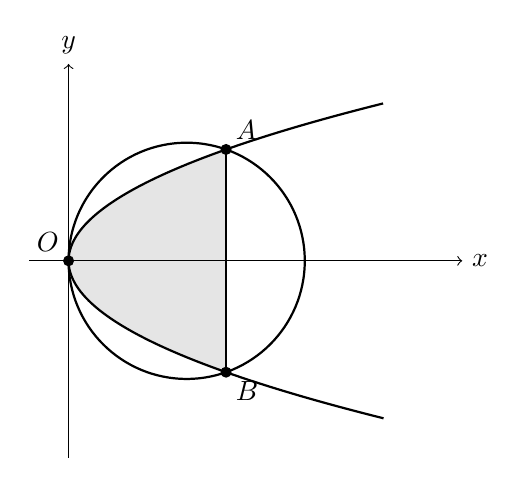
\begin{tikzpicture}
				% parameters
				\def\p{0.5}
				\def\R{1.5}

				% Intersection points
				% y^2 = 2px, (x-R)^2 + y^2 = R^2 => x^2 - 2Rx + 2px = 0 => x = 2(R-p)
				% y^2 = 2p * 2(R-p) => y = +/- sqrt(4p(R-p))
				\pgfmathsetmacro{\ymax}{sqrt(4*\p*(\R-\p))}
				\coordinate (A) at ({2*(\R-\p)}, \ymax);
				\coordinate (B) at ({2*(\R-\p)}, -\ymax);

				% Fill the area enclosed by chord AB and the parabola
				\fill[gray!20] (A) -- (B) -- plot[domain=-\ymax:\ymax, samples=100] ({\x*\x/(2*\p)}, \x) -- cycle;
				\draw[thick] (A) -- (B);

				% Draw axis
				\draw[->] (-0.5,0) -- (5,0) node[right] {$x$};
				\draw[->] (0,-2.5) -- (0,2.5) node[above] {$y$};

				% Draw curve y^2 = 2 p x
				\draw[thick] plot[domain=-2:2, samples=100] ({\x*\x/(2*\p)}, \x);

				% Draw circle (R, 0), R = p
				\draw[thick] (\R,0) circle (\R);
				
				\fill (A) circle (2pt) node[above right] {$A$};
				\fill (B) circle (2pt) node[below right] {$B$};
				\fill (0,0) circle (2pt) node[above left] {$O$};
			\end{tikzpicture}
		\end{figure}

		联立抛物线方程和圆的方程,解得:
		$$
		A\ab(2(R - p), 2 \sqrt{p(R - p)}),\ B\ab(2(R - p), -2 \sqrt{p(R - p)})
		$$
		那么所求面积为:
		$$
		\begin{aligned}
			A & = \int_{-2 \sqrt{p(R - p)}}^{2 \sqrt{p(R - p)}} \ab(2(R - p) - \frac{y^2}{2p}) \dd{y} \\
			& = \ab[2(R - p) y - \frac{y^3}{6p}]_{-2 \sqrt{p(R - p)}}^{2 \sqrt{p(R - p)}} \\
			& = \frac{16}{3} p^{\frac{1}{2}} (R - p)^{\frac{3}{2}}
		\end{aligned}
		$$
	\end{solution}
\end{problem}

\begin{problem}
	课后习题 8.1.4

	\begin{solution}
		\begin{figure}[H]
			\centering
			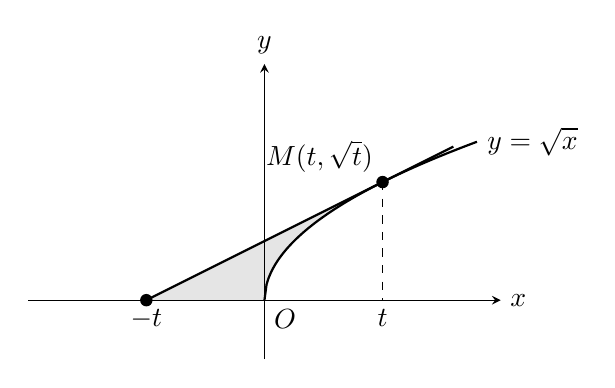
\begin{tikzpicture}[>=stealth, scale=1.5]
				% Define dynamic point M
				\def\xm{1}
				\pgfmathsetmacro{\ym}{sqrt(\xm)}
				\pgfmathsetmacro{\xt}{-\xm}

				% Fill area
				\fill[gray!20] (\xt,0) -- (\xm,\ym) -- plot[domain=\xm:0, samples=100] (\x, {sqrt(\x)}) -- (0,0) -- cycle;

				% Draw axes
				\draw[->] (-2,0) -- (2,0) node[right] {$x$};
				\draw[->] (0,-0.5) -- (0,2) node[above] {$y$};

				% Draw curve
				\draw[thick] plot[domain=0:1.8, samples=100] (\x, {sqrt(\x)}) node[right] {$y=\sqrt{x}$};

				% Draw tangent
				\draw[thick] (\xt, 0) -- ({\xm+0.6}, {\ym + 0.6/(2*sqrt(\xm))});

				% Annotations
				\fill (\xm,\ym) circle (1.5pt) node[above left] {$M(t, \sqrt{t})$};
				\fill (\xt,0) circle (1.5pt) node[below] {$-t$};
				\draw[dashed] (\xm,\ym) -- (\xm,0) node[below] {$t$};
				\node[below right] at (0,0) {$O$};
			\end{tikzpicture}
		\end{figure}

		设 $M\ab(t, \sqrt{t})$,那么易知切线方程为
		$$
		l: y = \frac{1}{2 \sqrt{t}} x + \frac{\sqrt{t}}{2}
		$$
		并且求得切线交 $x$ 轴于 $(-t, 0)$。

		用三角形面积减去曲线下方的面积,就得到所求面积:
		$$
		A = \frac{1}{2} \cdot \sqrt{t} \cdot 2t - \int_0^t \sqrt{x} \dd{x} = t^{\frac{3}{2}} - \ab[\frac{2}{3} x^\frac{3}{2}]_0^t = \frac{1}{3} t^{\frac{3}{2}}
		$$
		由题,$A = \frac{1}{3}$,因此 $t = 1$,$M(1, 1)$。
	\end{solution}
\end{problem}

\begin{problem}
	课后习题 8.1.5

	\begin{solution}
		\begin{figure}[H]
			\centering
			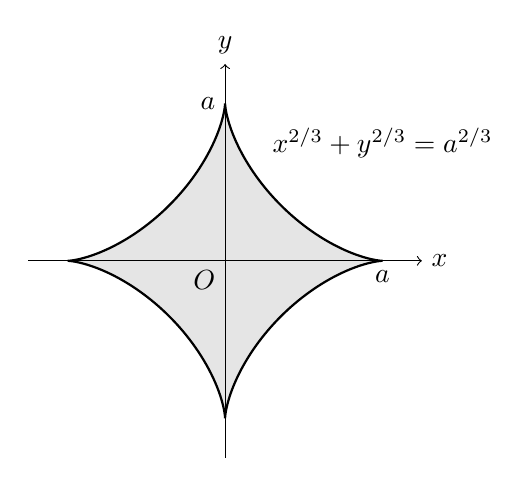
\begin{tikzpicture}[scale=1]
				\def\a{2}
				
				% Draw astroid
				\draw[thick, domain=0:360, samples=200, smooth, variable=\t, fill=gray!20] 
					plot ({\a*(cos(\t))^3}, {\a*(sin(\t))^3});

				% Draw axes
				\draw[->] (-2.5,0) -- (2.5,0) node[right] {$x$};
				\draw[->] (0,-2.5) -- (0,2.5) node[above] {$y$};                
				
				% Labels
				\node at (2, 1.5) {$x^{2/3} + y^{2/3} = a^{2/3}$};
				\node[below left] at (0,0) {$O$};
				\node[below] at (\a, 0) {$a$};
				\node[left] at (0, \a) {$a$};
			\end{tikzpicture}
		\end{figure}

		将曲线表示为参数方程:
		$$
		\begin{cases}
			x = a \cos^3 t \\
			y = a \sin^3 t
		\end{cases}, \quad t \in [0, 2\pi]
		$$

		因为曲线的对称性,我们先计算 $t \in [0, \frac{\pi}{2}]$ 的面积。考虑使用微元法。当 $t$ 有微小增量 $\dd t$ 时,有:
		$$
		\dd V = \frac{1}{2} (x (y + \dd y) - (x + \dd x) y) = \frac{1}{2} (x \dd y - y \dd x)
		$$

		那么:
		$$
		\begin{aligned}
			A_1 & = \int_0^{\pi/2} a \cos^3 t \cdot 3a \cos t \sin^2 t \dd{t} \\
			& = 3a^2 \int_0^{\pi/2} \cos^4 t \sin^2 t \dd{t} \\
			& = 3a^2 \int_0^{\pi/2} \cos^4 t (1 - \cos^2 t) \dd{t} \\
			& = 3a^2 \ab(\int_0^{\pi/2} \cos^4 t \dd{t} - \int_0^{\pi/2} \cos^6 t \dd{t}) \\
			& = 3a^2 \ab(\frac{3 \cdot 1}{4 \cdot 2} \cdot \frac{\pi}{2} - \frac{5 \cdot 3 \cdot 1}{6 \cdot 4 \cdot 2} \cdot \frac{\pi}{2}) = \frac{3 \pi}{32} a^2 \\
			A_2 & = \int_0^{\pi/2} a \sin^3 t \cdot \ab(-3a \sin t \cos^2 t) \dd{t} = -\frac{3 \pi}{32} a^2 
		\end{aligned}
		$$
		最终整个图形的面积为:
		$$
		A = 4 \cdot \frac{1}{2}(A_1 - A_2) = \frac{3 \pi}{8} a^2
		$$
	\end{solution}
\end{problem}

\begin{problem}
	课后习题 8.1.8

	\begin{solution}
		\begin{figure}[H]
			\centering
			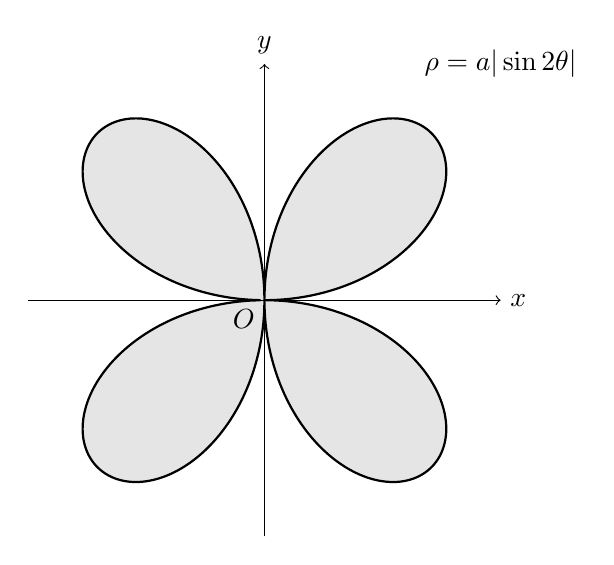
\begin{tikzpicture}[scale=1.5]
				\def\a{2}
				
				% Fill area
				\fill[gray!20, domain=0:360, samples=200, smooth, variable=\t] 
					plot ({\a*abs(sin(2*\t))*cos(\t)}, {\a*abs(sin(2*\t))*sin(\t)});

				% Draw axes
				\draw[->] (-2,0) -- (2,0) node[right] {$x$};
				\draw[->] (0,-2) -- (0,2) node[above] {$y$};
				
				% Draw curve
				\draw[thick, domain=0:360, samples=300, smooth, variable=\t] 
					plot ({\a*abs(sin(2*\t))*cos(\t)}, {\a*abs(sin(2*\t))*sin(\t)});
				
				% Labels
				\node at (2, 2) {$\rho = a |\sin 2 \theta|$};
				\node[below left] at (0,0) {$O$};
			\end{tikzpicture}
		\end{figure}

		曲线是对称的,先计算 $\theta \in [0, \frac{\pi}{2}]$ 的面积:
		$$
		\begin{aligned}
			A' & = \int_0^{\pi/2} \frac{1}{2} \rho^2 \,\dd \theta = \frac{a^2}{2} \int_0^{\pi/2} \sin^2 2\theta \,\dd \theta \\
			& = \frac{a^2}{2} \int_0^{\pi/2} \frac{1 - \cos 4\theta}{2} \,\dd \theta \\
			& = \frac{a^2}{2} \ab[\frac{1}{2} \theta - \frac{1}{8} \sin 4\theta]_0^{\pi/2} = \frac{\pi}{8} a^2
		\end{aligned}
		$$

		整个曲线的面积为 $A = 4 A' = \frac{\pi}{2} a^2$。
	\end{solution}
\end{problem}

\begin{problem}
	课后习题 8.2.2

	\begin{solution}
		$$
		V = \int_0^8 \pi y^{\frac{2}{3}} \dd{y} = \pi \ab[\frac{3}{5} y^{\frac{5}{3}}]_0^8 = \frac{32}{5} \pi
		$$
	\end{solution}
\end{problem}

\begin{problem}
	课后习题 8.2.4

	\begin{solution}
		先考虑 $x \ge 0$ 的部分,此时 $t \in [0, \frac{\pi}{2}]$。对 $x$ 轴方向做微元法,那么在 $t$ 有微小增量 $\dd t$ 时,圆盘半径为 $y$,高为 $\dd x$,于是有:
		$$
		\begin{aligned}
			V' & = \int_0^{\pi/2} \pi \ab(a \sin^3 t)^2 \cdot 3a \sin t \cos^2 t \dd t \\
			& = 3a^3 \int_0^{\pi/2} \sin^7 t \cos^2 t \dd t \\
			& = 3a^3 \int_0^{\pi/2} \sin^7 t (1 - \sin^2 t) \dd t \\
			& = 3a^3 \ab(\int_0^{\pi/2} \sin^7 t \dd t - \int_0^{\pi/2} \sin^9 t \dd t) \\
			& = 3a^3 \ab(\frac{6 \cdot 4 \cdot 2}{7 \cdot 5 \cdot 3} - \frac{8 \cdot 6 \cdot 4 \cdot 2}{9 \cdot 7 \cdot 5 \cdot 3}) = \frac{16}{105} a^3
		\end{aligned}
		$$

		那么整个曲线的体积为 $V = 2V' = \frac{32}{105} a^3$。
	\end{solution}
\end{problem}

\begin{problem}
	课后习题 8.2.5

	\begin{solution}
		$$
		\begin{aligned}
			V & = \int_{-1}^1 \pi \ab(\ab(2 + \sqrt{1 - y^2})^2 - \ab(2 - \sqrt{1 - y^2})^2) \dd{y} \\
			& = \pi \int_{-1}^1 8 \sqrt{1 - y^2} \dd{y} \\
			& = 8 \pi \cdot \pi = 8\pi^2
		\end{aligned}
		$$
	\end{solution}
\end{problem}

\begin{problem}
	课后习题 8.2.7

	\begin{solution}
		由题可得,切线为 $y = \frac{1}{\E} x$,切点为 $(\E, 1)$。

		\begin{itemize}
			\item 对于切线围出的部分:
			$$
			V_1 = \int_0^\E \pi \ab(\frac{1}{\E} x)^2 \dd{x} = \frac{\pi}{\E^2} \ab[\frac{1}{3} x^3]_0^\E = \frac{\pi \E}{3}
			$$
			\item 对于 $y = \ln x$ 围出的部分:
			$$
			V_2 = \int_1^\E \pi \ln^2 x \dd{x} = \pi \ab[2x - 2x \ln x - x \ln^2 x]_1^\E = (\E - 2) \pi
			$$
		\end{itemize}
		
		因此,整个图形的体积为 $V = V_1 - V_2 = \ab(2 - \frac{2}{3} \E) \pi$。
	\end{solution}
\end{problem}

\begin{problem}
	课后习题 8.2.8

	\begin{solution}
		$$
		\begin{aligned}
			V & = \frac{2\pi}{3} \int_0^\pi \ab(a (1 - \cos \theta))^3 \sin \theta \,\dd \theta \\
			& = \frac{2\pi}{3} \int_0^\pi a^3 (1 - \cos \theta)^3 \,\dd (1 - \cos \theta) \\
			& = \frac{2\pi}{3} \ab[\frac{a^3}{4} (1 - \cos \theta)^4]_0^\pi = \frac{8\pi}{3} a^3
		\end{aligned}
		$$
	\end{solution}
\end{problem}

\begin{problem}
	课后习题 8.2.9

	\begin{solution}
		平面 $x = x_0$ 截图形得到的是椭圆 $\frac{y^2}{b^2} + \frac{z^2}{c^2} = 1 - \frac{x_0^2}{a^2}$,其面积 $S = \pi b c \ab(1 - \frac{x_0^2}{a^2})$。
		$$
		\begin{aligned}
			V & = \int_{-a}^a \pi b c \ab(1 - \frac{x^2}{a^2}) \dd{x} = \pi b c \int_{-a}^a \ab(1 - \frac{x^2}{a^2}) \dd x \\
			& = \pi b c \ab[x - \frac{1}{3a^2} x^3]_{-a}^a = \frac{4\pi a b c}{3}
		\end{aligned}
		$$
	\end{solution}
\end{problem}

\begin{problem}
	课后习题 8.2.10

	\begin{solution}
		\begin{itemize}
			\item[\textbf{3)}] 将曲线参数化:
			$$
			\begin{cases}
				x = 2 \cos t \\
				y = \sin t
			\end{cases}, \quad t \in [0, 2\pi]
			$$
			那么根据公式,旋转曲面面积为:
			$$
			\begin{aligned}
				A & = 2\pi \int_{-\pi/2}^{\pi/2} 2 \cos t \sqrt{4 \sin^2 t + \cos^2 t} \dd{t} \\
				& = 4\pi \int_{-\pi/2}^{\pi/2} \sqrt{3 \sin^2 t + 1} \,\dd (\sin t) \\
				& = 4\sqrt{3} \pi \int_{-1}^1 \sqrt{u^2 + \frac{1}{3}} \dd{u} \\
				& = 4\sqrt{3} \pi \ab[\frac{u}{2} \sqrt{u^2 + \frac{1}{3}} + \frac{1}{6} \ln \ab(u + \sqrt{u^2 + \frac{1}{3}})]_{-1}^1 \\
				& = 4\pi \ab(2 + \frac{1}{\sqrt{3}} \ln \ab(2 + \sqrt{3}))
			\end{aligned}
			$$

			\item[\textbf{4)}] 曲线方程化为 $y = \frac{x^2}{4}$,那么:
			$$
			\begin{aligned}
				A & = 2\pi \int_0^2 x \sqrt{1 + \ab(\frac{x}{2})^2} \dd{x} \\
				& = \pi \int_0^2 \sqrt{1 + \frac{x^2}{4}} \,\dd (x^2) \\
				& = \frac{\pi}{2} \int_0^4 \sqrt{4 + u} \dd{u} \\
				& = \frac{\pi}{2} \ab[\frac{2}{3} (4 + u)^{\frac{3}{2}}]_0^4 = \frac{8\pi}{3} \ab(2 \sqrt{2} - 1)
			\end{aligned}
			$$
		\end{itemize}
	\end{solution}
\end{problem}

\begin{problem}
	课后习题 8.2.11

	\begin{solution}
		由题知,切线为 $l: y = \frac{1}{2} x$,切点为 $(2, 1)$。

		\begin{itemize}
			\item 对于切线形成的面积:
			$$
			A_1 = 2\pi \int_0^2 \frac{1}{2} x \sqrt{1 + \ab(\frac{1}{2})^2} \dd{x} = \frac{\sqrt{5} \pi}{2} \int_0^2 x \dd{x} = \sqrt{5} \pi
			$$

			\item 对于曲线形成的面积:
			$$
			\begin{aligned}
				A_2 & = 2\pi \int_1^2 \sqrt{x - 1} \sqrt{1 + \ab(\frac{1}{2 \sqrt{x - 1}})^2} \dd{x} \\
				& = \pi \int_1^2 \sqrt{4x - 3} \dd{x} \\
				& = \pi \ab[\frac{1}{6} (4x - 3)^{\frac{3}{2}}]_1^2 = \frac{(5 \sqrt{5} - 1)\pi}{6}
			\end{aligned}
			$$
		\end{itemize}
	\end{solution}
\end{problem}

\begin{problem}
	课后习题 8.2.13

	\begin{solution}
		\begin{itemize}
			\item[\textbf{1)}]
			$$
			\begin{aligned}
				A & = 2\pi \int_0^\pi r \sin \theta \cdot \sqrt{r^2 + r'^2} \,\dd \theta \\
				& = 2\pi \int_0^\pi 2 a^2 (1 - \cos \theta) \sin \theta \sin \frac{\theta}{2} \,\dd \theta \\
				& = 2\pi \int_0^\pi 2 a^2 \cdot 2 \sin^2 \frac{\theta}{2} \cdot 2 \sin \frac{\theta}{2} \cos \frac{\theta}{2} \cdot \sin \frac{\theta}{2} \,\dd \theta \\
				& = 32\pi a^2 \int_0^\pi \sin^4 \frac{\theta}{2} \,\dd(\sin \frac{\theta}{2}) \\
				& = 32\pi a^2 \ab[\frac{1}{5} \sin^5 \frac{\theta}{2}]_0^\pi = \frac{32\pi}{5} a^2
			\end{aligned}
			$$

			\item[\textbf{2)}] 曲线如图:

			\begin{figure}[H]
				\centering
				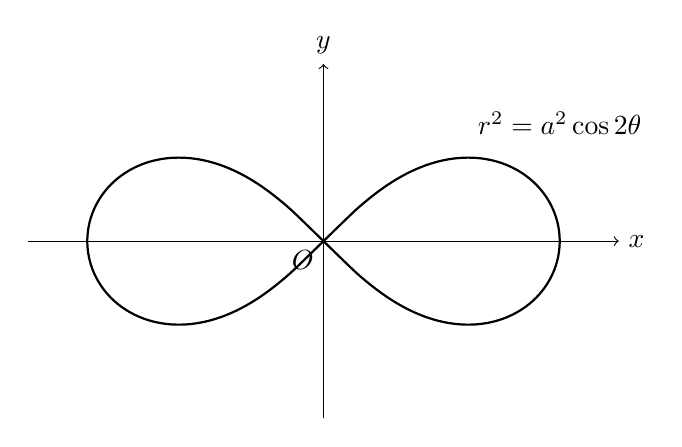
\begin{tikzpicture}[scale=1.5]
					\def\a{2}
					
					% Draw axes
					\draw[->] (-2.5,0) -- (2.5,0) node[right] {$x$};
					\draw[->] (0,-1.5) -- (0,1.5) node[above] {$y$};
					
					% Draw lemniscate
					% Right loop: -45 to 45
					\draw[thick, domain=-45:45, samples=100, smooth, variable=\t] 
						plot ({\a*sqrt(cos(2*\t))*cos(\t)}, {\a*sqrt(cos(2*\t))*sin(\t)});
					% Left loop: 135 to 225
					\draw[thick, domain=135:225, samples=100, smooth, variable=\t] 
						plot ({\a*sqrt(cos(2*\t))*cos(\t)}, {\a*sqrt(cos(2*\t))*sin(\t)});
						
					% Labels
					\node at (2, 1) {$r^2 = a^2 \cos 2\theta$};
					\node[below left] at (0,0) {$O$};
				\end{tikzpicture}
			\end{figure}
			
			对曲线方程两侧求导:
			$$
			2r r' = 2a^2 \sin 2\theta \Rightarrow r' = \frac{a^2 \sin 2\theta}{r}
			$$
			再代入 $r = a \sqrt{\cos 2\theta}$ 得到:
			$$
			r' = \frac{a \sin 2\theta}{\sqrt{\cos 2\theta}}
			$$
			最后求面积:
			$$
			\begin{aligned}
				A & = 2 \cdot 2\pi \int_0^{\pi/4} r \sin \theta \cdot \sqrt{r^2 + r'^2} \,\dd \theta \\
				& = 4\pi \int_0^{\pi/4} a \sqrt{\cos 2\theta} \sin \theta \sqrt{a^2 \cos 2\theta + \frac{a^2 \sin^2 2\theta}{\cos 2\theta}} \,\dd \theta \\
				& = 4\pi a^2 \int_0^{\pi/4} \sin \theta \,\dd \theta \\
				& = 4\pi a^2 \ab[-\cos \theta]_0^{\pi/4} = 2(2 - \sqrt{2}) \pi a^2
			\end{aligned}
			$$
		\end{itemize}
	\end{solution}
\end{problem}